% Created 2015-10-23 Fri 12:55
\documentclass{scrartcl}
\usepackage[utf8]{inputenc}
\usepackage[T1]{fontenc}
\usepackage{fixltx2e}
\usepackage{graphicx}
\usepackage{longtable}
\usepackage{float}
\usepackage{wrapfig}
\usepackage{soul}
\usepackage{textcomp}
\usepackage{marvosym}
\usepackage{wasysym}
\usepackage{latexsym}
\usepackage{amssymb}
\usepackage{hyperref}
\tolerance=1000
\usepackage{khpreamble}
\newcommand{\tustin}{\frac{2}{h}\frac{z-1}{z+1}}
\providecommand{\alert}[1]{\textbf{#1}}

\title{Computerized control - partial exam 2 (dummy)}
\author{Kjartan Halvorsen}
\date{2015-10-16}
\hypersetup{
  pdfkeywords={},
  pdfsubject={},
  pdfcreator={Emacs Org-mode version 7.9.3f}}

\begin{document}

\maketitle





\section*{Problem 1}
\label{sec-1}

Figure \ref{fig:step} shows the step response of the system 
\[ G(s) = \frac{1}{(s+1)^2(s+3)} \]
for an experiment to determine the ultimate gain and ultimate period.
\begin{figure}
\begin{center}
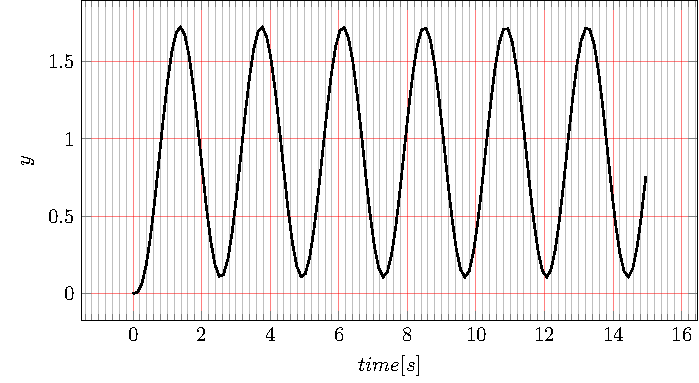
\includegraphics[]{ultimate_gain_experiment}
\caption{Response of closed-loop system using proportional control with gain equal to the ultimate gain.}
\label{fig:step}  
\end{center}
\end{figure}

  \textbf{(a)} What is the ultimate period and the phase-crossover frequency?

  \textbf{(b)} Use the transfer function and the phase-crossover frequency to determine the ultimate gain.

  \textbf{(c)} Determine a suitable continuous-time PID-controller using table 8.3 from Å\&W.

  \textbf{(d)} Obtain a sampled controller by using the backward difference for the D-part and Tustin's approximation for the I-part of the PID-controller.
\section*{Solutions}
\label{sec-2}

  \textbf{(a)} 
  \begin{center}
  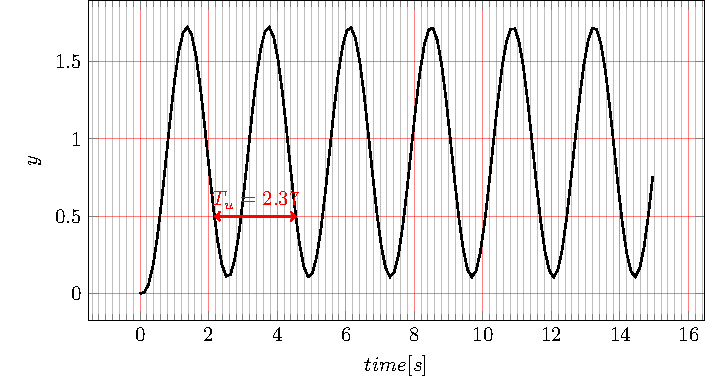
\includegraphics[]{ultimate_gain_experiment-solution}
  \end{center}
  The phase-crossover frequency is $\omega_p = \frac{2\pi}{T_u} = 2.65$ 

  \textbf{(b)}
  We know that the phase-crossover frequency is $2.65$ and that at this frequency the Nyquist curve of the open-loop transfer function crosses the negative real axis. Multiplying the transfer function $G(s)$ by the ultimate gain $K_u$ causes the Nyquist curve to cross the negative real axis at -1 (that is why there are self-sustained oscillations). We get
  \[ |K_uG(i\omega_p)| &= 1 \] or
  \begin{align*}
  K_u &= \frac{1}{|G(i\omega_p)|} = |i\omega_p + 1|^2|i\omega_p+3|\\
     &= (\omega_p^2 + 1)\sqrt{\omega_p^2 + 9} \approx 32.11
  \end{align*}

  \textbf{(c)} The controller parameters become 
  \[ K_p = 0.6K_u = 19.27, \quad T_i = 0.5T_u = 1.185, \quad T_d = 0.125T_u = 0.296 \]

  \textbf{(d)}
  The controller is
  \begin{align*}
  F_d(z) &= K_p + \frac{K_p}{T_i s' } |_{s'= \tustin{}} + K_pT_ds'|_{s'= \frac{z-1}{zh}}\\ 
         &= K_p + \frac{K_p}{T_i\tustin{}} + \frac{K_pT_d(z-1)}{zh}\\
         &= K_p + \frac{K_ph(z+1)}{T_i(z-1)} + \frac{K_pT_d(z-1)}{zh}
  \end{align*}


  

\end{document}
